\documentclass[12pt,prb,aps,epsf]{report}
\usepackage[utf8]{inputenc}
\usepackage{amsmath}
\usepackage{amsfonts}
\usepackage{amssymb}
\usepackage{graphicx} 
\usepackage{latexsym} 
\usepackage[toc,page]{appendix}
\usepackage{listings}
\usepackage{xcolor}
\usepackage{soul}
\usepackage[T1]{fontenc}
\usepackage{amsthm}
\usepackage{mathtools}
\usepackage{setspace}
\usepackage{array,multirow,makecell}
\usepackage{geometry}
\usepackage{textcomp}
\usepackage{float}
%\usepackage{siunitx}
\usepackage{cancel}
%\usepackage{tikz}
%\usetikzlibrary{calc, shapes, backgrounds, arrows, decorations.pathmorphing, positioning, fit, petri, tikzmark}
\usepackage{here}
\usepackage{titlesec}
%\usepackage{bm}
\usepackage{bbold}

\geometry{hmargin=2cm,vmargin=2cm}

\begin{document}
	
	\title{LP 14 Machines thermiques réelles}
	\author{Naïmo Davier}
	
	\maketitle
	
	\tableofcontents
	
	\pagebreak
	
	
\subsection{Pré-requis}
Premier et second principes de la thermodynamique.

\section{Introduction}

On ne se rend pas toujours compte aujourd'hui de l'omniprésence des machines thermiques, et d'à quel point il était laborieux de fonctionner sans elles. Si on regarde 200 ans en arrière, la nécessité s'est posée de trouver un moyen d'enlever l'eau des mines, autre qu'avec des seaux portés à la main... Pour ce faire on a d'abord pensé à utiliser la pression atmosphérique : on fait le vide dans un cylindre puis on laisse ensuite la pression atmosphérique enfoncer le piston. La question est : "comment faire le vide ?" Ces questions et réflexions très pratiques sont en fait à l'origine de la thermodynamique qui est une science induite par les technologies dont elle s'est évertuée à expliquer formaliser le fonctionnement.\\
Nous allons ici partir des principes maintenant bien connus de la thermodynamique pour expliquer le fonctionnement des moteurs thermiques.

\section{Machines thermiques idéales}
Voir DGLR p 103, Faroux-Renault p 175, et le Latour pour cette partie.
\subsection{Machine thermique}

Une machine est un système qui effectue une même transformation cyclique encore et encore, c'est à dire qu'au bout d'un cycle le système se retrouve dans son état de départ, et peut ainsi recommencer un nouveau cycle identique au précédent.\\
Si cette machine reçoit de l'extérieur du travail mécanique et de la chaleur on la qualifie de thermique, tandis que si de plus elle fournit du travail à l'extérieur alors on parlera de moteur thermique.\\

Lors d'un cycle effectué par la machine considérée, on aura, selon le premier principe 
\begin{eqnarray}
\Delta U =  W + Q = 0
\end{eqnarray}
et selon le second principe 
\begin{eqnarray}
\Delta S = 0 \geq \oint \frac{\delta Q}{T^{ext}}
\end{eqnarray}
puisque U et S étant des fonctions d'état, leur variation est nulle pendant un cycle.

\paragraph{Remarque} On peut montrer à partir de ces deux relations qu'il n'existe pas de mouvement perpétuel de première espèce, et que le second principe peut être formulé grâce à l'énoncé de Clausius : "il est impossible de réaliser un processus dont le seul résultat serait le transfert d'une quantité de chaleur d'un corps plus froid à un corps plus chaud". (V DGLR p 104)\\

Ces relations nous montrent que dans le cas d'un moteur c'est à dire si $W < 0$, alors cela impose $Q > 0$, il faut donc vérifier simultanément 
\begin{eqnarray}
Q > 0 \hspace{1cm}\mathrm{et} \hspace{1cm} \oint \frac{\delta Q}{T^{ext}} \leq 0
\end{eqnarray} 
ce qui n'est pas possible avec une unique source de chaleur, ou différentes sources fournissant toutes de la chaleur ($Q_i >0$) puisque par définition $T^{ext}$ est toujours positive. Il est donc impossible de former un processus qui transforme intégralement une quantité de chaleur en travail.\\
Cela ne signifie pas pour autant que l'on ne puisse pas former de motheur thermique comme nous allons le voir maintenant.

\subsection{Machine de Carnot}

Le moteur le plus simple conceptuellement est donc ditherme : il fonctionne en contacte avec deux sources, une chaude et une froide.\\
Si on considère donc le cas d'une machine ditherme, avec deux thermostats de températures différentes $T_c$ et $T_f$ avec $T_c>T_f$, on a ainsi
\begin{eqnarray}
Q_c = -W - Q_f\\
\frac{Q_f}{T_f} + \frac{Q_c}{T_c} \leq 0 \label{5}
\end{eqnarray}
selon le premier et le second principe. Ces relations permettent de tracer le diagramme de Raveau où on représente $Q_c$ en fonction de $Q_f$. 
\begin{figure}[h]
	\centerline{ \includegraphics[width=11cm]{raveau} }
\end{figure}
On y voit qu'il y a deux parties intéressantes, la partie (2) qui correspondra aux machines frigorifiques, et la partie (1) où$W>0$ qui correspond donc au cas d'un moteur. On peut remarquer dans ce cas qu'il faut que $Q_c>0$ et de même que $Q_f<0$. Il y a donc, pour un moteur ditherme, nécessairement une source à laquelle on fournit de la chaleur.
Un tel moteur ditherme idéal, si il fonctionne de manière réversible, est appelé moteur de Carnot. On peut représenter le cycle qu'il décrit sur un diagramme (P,V) ou (S,T).
\begin{figure}[h]
	\centerline{ \includegraphics[width=15cm]{cycle_carnot} }
\end{figure}

Ce cycle est constitué par 
\begin{itemize}
	\item une détente isotherme à la température $T_c$ (M $\rightarrow$ N) où la machine absorbe une quantité de de chaleur $Q_c$
	\item une détente adiabatique
	\item une compression isotherme à la température $T_f$ où le système cède une énergie $|Q_f|$ à la la source froide
	\item une compression adiabatique
\end{itemize}
Le cycle représenté ici est un cycle moteur : on le voit car il est parcouru dans le plan (P,V) dans le sens des aiguilles d'une montre.\\
Le travail fournit à l'extérieur est alors l'aire du cycle 
\begin{eqnarray}
W = \oint \delta W = \oint PdV \stackrel{ici}{=} \int_M^N PdV + \int _N^P PdV - \int_Q^P PdV - \int _M^Q pdV > 0
\end{eqnarray}
(attention on calcule ici le travail reçu par l'extérieur, il est donc normal d'obtenir un travail positif pour un moteur).

\subsection{Rendement}
Le rendement, noté $\eta$ est défini de manière assez intuitive comme l'énergie reçue/utile divisée par l'énergie fournie/dépensée, dans le cas d'un moteur ditherme on aura donc 
\begin{eqnarray}
\eta = \frac{-W}{Q_c} = 1 +\frac{Q_f}{Q_c}.
\end{eqnarray}
Il est assez naturel d'en déduire le théorème de Carnot qui nous dit que le rendement réel sera toujours inférieur à un rendement idéal correspondant au cas d'un cycle réversible qui s'exprime comme 
\begin{eqnarray}
\eta^{rev} = 1 - \frac{T_f}{T_c}.
\end{eqnarray}
On le démontre à partir de l'expression du rendement et du second principe qui nous donne 
\begin{eqnarray}
\frac{Q_f}{T_f} + \frac{Q_c}{T_c} \leq 0 \; \Longrightarrow \; \frac{Q_f}{Q_c} \leq \frac{T_f}{T_c}.
\end{eqnarray}
On voit donc qu'un écart de température maximal entre les sources de chaleur permettra un rendement optimal.\\

Il est possible d'étendre ce résultat au cas général : le rendement sera optimal lorsque la création d'entropie durant un cycle sera minimale, cette dernière ne pouvant diminuer, le rendement sera optimal lorsque l'entropie demeure constante c'est à dire lorsque le cycle est réversible.\\

Toutes ces considérations nous ont permis d'introduire le concept de moteur thermique, mais nous somme resté dans un cadre très théorique et idéal, on se propose maintenant d'appliquer les éléments introduits au cas de moteurs et de machines thermiques réelles. 

\section{Moteurs réels}
Voir Faroux-Renault p179 et le Latour pour cette partie.

\subsection{Moteur à explosion}

On va ici étudier le fonctionnement du moteur à explosion à quatre temps (couramment appelé moteur à essence) qui équipe notamment une partie de nos voitures et certains avions. On peut décrire son cycle par temps, un temps étant un déplacement du piston de la position morte haute à la position morte basse ou inversement.
\begin{itemize}
	\item Admission : partant du point mort haut, le piston, entrainé par le vilebrequin, descend en aspirant un mélange-air essence jusqu'au point mort bas, ce que l'on considère par la suite comme une isobare.
	\item Compression : le piston remonte en compressant le mélange. On va la considérer comme étant adiabatique.
	\item Explosion-détente : une étincelle provoque l'explosion du mélange ce qui repousse le piston au point mort bas, c'est la phase motrice. On modélise cette partie avec une compression isochore suivie d'une détente adiabatique.
	\item Échappement : le piston remonte et chasse alors les gaz d'échappement par la soupape, ce qu'on assimile à une isochore ce qui suppose que le gaz refroidit instantanément. Le cycle peut ensuite recommencer.
\end{itemize}
\begin{figure}[h]
	\centerline {\includegraphics[width=9cm]{moteur_4_temps}
				\includegraphics[width=9cm]{cycle_explosion} }
\end{figure}
Le système que l'on considère ici est le gaz à l'intérieur du cylindre, on peut considérer qu'il est fermé puisque les deux phases d'échanges de matière n'influe pas sur le travail (aller retour à p constante). On assimile de plus ce gaz à un gaz parfait et on fait comme si sa constitution ne variait pas lors de l'explosion, ce qui revient à Ces hypothèses vont nous permettre de mener une analyse formelle, qui serait compliquée si ce n'est impossible si nous ne les faisions pas.\\
On peut noter que dans notre modèle le cycle est constitué par ABCDA puisque l'autre partie ne correspond à aucun échange de chaleur ou de travail. On peut donc estimer un rendement sur ce cycle, on considère pour les portions BC et DA que le système reçoit de la chaleur, bien que dans le premier ce soit la combustion qui libère de la chaleur. On a donc formellement 
\begin{eqnarray}
Q_1 = \int_{T_B}^{T_C} m c_v dT = mc_v (T_C-T_B) \hspace{1cm}\mathrm{et}\hspace{1cm} Q_2 = \int_{T_D}^{T_A} m c_v dT = mc_v (T_A-T_D)
\end{eqnarray}
en supposant que la capacité thermique $mc_v$ ne dépende pas de la température. On en déduit l' expression suivante pour le rendement 
\begin{eqnarray}
\eta = \frac{-W}{Q_1} = \frac{Q_1+Q_2}{Q_1} = 1 + \frac{Q_2}{Q_1} = 1 + \frac{T_A-T_D}{T_C-T_B}
\end{eqnarray}
On peut alors utiliser la relation de Laplace pour les gaz parfait $TV^{\gamma-1}=cste$ dans le cas des deux adiabatiques 
\begin{eqnarray}
\left(\frac{V_A}{V_B}\right)^{\gamma-1} = a^{\gamma-1} = \frac{T_B}{T_A} = \frac{T_C}{T_D}
\end{eqnarray} où on a introduit le rapport volumétrique $a = \frac{V_A}{V_B} = \frac{V_D}{V_C}$, pour réécrire 
\begin{eqnarray}
\frac{T_A-T_D}{T_C-T_B} = \frac{T_B a ^{1-\gamma} - T_Ca^{1-\gamma}}{T_C-T_B} = - a^{1-\gamma}
\end{eqnarray}
ce qui nous donne finalement 
\begin{eqnarray}
\eta = 1 - a ^{1-\gamma}
\end{eqnarray}
On voit que le rendement sera optimal pour $a$ très grand (en prenant $\gamma=1,4$), dans la pratique on est limité car plus $a$ est grand plus la pression montera haut, et il faut donc avoir des matériaux plus résistant donc à priori plus cher et plus lourds, on cherche donc un compromis. On peut estimer ce rendement théorique en prenant a = 9 (ce qui est une valeur habituelle) et $\gamma = 1,4$ (cas de l'air), on trouve alors $58,8\%$, ce rendement est cependant associé à un modèle très idéalisé. Il possible de suivre le cycle réel (dit cycle de Beau de Rochas) en utilisant l'indicateur de Watt. On obtient alors un cycle ayant une l'allure suivante 
\begin{figure}[h]
	\centerline{\includegraphics[width=10cm]{cycle_beau_de_rochas}}
\end{figure}
dont on peut déduire le travail fournit en soustrayant les aires des cycles, en comptant positivement celui parcouru dans le sens des aiguilles d'une montre. On peut calculer le rendement en estimant $Q_1$ grâce en se basant sur le pouvoir calorifique du carburant, on trouve alors qu'il ne dépasse pas $35\%$, et il est encore plus faible si on considère que le rendement pratique obtenu en regardant la puissance obtenue aux roues motrices sur la puissance calorifique du carburant, cela étant dû à la nécessité d'entrainer d'autres organes du véhicule et aux pertes dues à la transmission.


\subsection{Moteur Diesel}
On veut maintenant se pencher sur l'autre type de moteur équipant nos voitures, où la différence majeure est que cette fois la combustion ne se fait pas à volume mais à pression constante.
On a dans le cas du moteur diesel un cycle du type 
\begin{figure}[h]
	\centerline {\includegraphics[width=9cm]{cycle_diesel}
				\includegraphics[width=9cm]{cycle_diesel_reel}}
\end{figure} 

Il est composé et peut être modélisé par
\begin{itemize}
	\item d'une admission mais cette fois d'air uniquement,
	\item d'une compression, supposée ici adiabatique,
	\item d'une combustion : le combustible est injecté sous pression et s'enflamme spontanément à la température résultant de la compression, ce qui repousse progressivement le piston, phase modélisée par une isobare,
	\item d'une détente à nouveau supposée adiabatique après que la combustion soit terminée,
	\item et enfin d'une phase d'échappement des gaz, modélisée par une isochore
\end{itemize}


Si on veut à nouveau faire une estimation du rendement associé à notre modèle on a 
\begin{eqnarray}
\eta = \frac{-W}{Q_1} = \frac{Q_1 + Q_2}{Q_1} = 1 + \frac{Q_2}{Q_1}
\end{eqnarray}
or 
\begin{eqnarray}
Q_1 = \int_B^C m C_p dT = mC_p(T_C-T_B) \hspace{1cm}\mathrm{et} \hspace{1cm} Q_2 = \int_D^A m C_v dT = mC_v(T_A-T_D)
\end{eqnarray}
donc on a 
\begin{eqnarray}
\frac{Q_1}{Q_2} = \frac{C_v}{C_p}\frac{T_A-T_D}{T_C-T_B} = \gamma^{-1}\frac{T_A-T_D}{T_C-T_B}
\end{eqnarray}
Les informations dont nous disposons pour évaluer le rendement sont :
\begin{itemize}
	\item on a une adiabatique de A à B donc : $\frac{T_A}{T_B} = \left(\frac{V_A}{V_B}\right)^{1-\gamma} = a^{1-\gamma}$,
	\item on a une deuxième adiabatique de C à D donc $\frac{T_D}{T_C} = \left(\frac{V_D}{V_C}\right)^{1-\gamma} = b^{1-\gamma}$,
	\item on a une isobare de B à C, et donc $P=cste$, ce qui mène, si on considère le mélange gaz-combustible comme un gaz parfait à $\frac{V_C}{T_C} = \frac{V_B}{T_B} \Rightarrow \frac{T_B}{T_C} = \frac{V_B}{V_C} = \frac{b}{a}$ puisque $V_D=V_A$ car on a une isochore entre D et A.
\end{itemize}
On en déduit 
\begin{eqnarray}
\frac{T_A-T_D}{T_C-T_B} = \frac{T_B a^{1-\gamma} - T_C b^{1-\gamma}}{T_C-T_B} = \frac{b\,a^{-\gamma} -  b^{1-\gamma}}{1-b/a} = -\frac{a^{-\gamma} -  b^{-\gamma}}{a^{-1}-b^{-1}}
\end{eqnarray}
et donc finalement que 
\begin{eqnarray}
\eta = 1 - \gamma^{-1} \frac{a^{-\gamma} -  b^{-\gamma}}{a^{-1}-b^{-1}}
\end{eqnarray}
Il n'est pas évident face à l'expression de ce rendement de dire comment il faut choisir a et b afin de l'optimiser, on peut donc le tracer pour $\gamma = 1,4$ (correspond à de l'air) et $a=10$ par exemple, on voit alors que $b = a$ sera optimal (on a par définition $b \leq a$) mais que l'on est proche du rendement maximum à $a$ donné pour un b plus faible. On voit aussi sur le diagramme (P,T) qu'une augmentation de b augmente bel et bien l'aire du cycle, mais de moins en moins, donc là encore il faut trouver un compromis puisque aune augmentation de b correspond à une augmentation du carburant consommé lors d'un cycle.
\begin{figure}[h]
	\centerline {\includegraphics[width=15cm]{rendement_diesel}}
\end{figure} 

\subsubsection{Discussion}
On peut maintenant discuter les avantages et inconvénients de ces deux types de moteurs.\\

Le moteur à explosion est plus rapide : un cycle met moins de temps à se faire, ce qui signifie que le moteur sera plus nerveux. Par contre on a peu de liberté au niveau pratique quand à la valeur du rapport volumétrique, et quand à la géométrie, car l'explosion ne doit se produire que lorsque le piston est en position haute, sinon on casse la bielle. De l'autre coté, le diesel permet plus de marge quand au choix du rapport volumétrique, et, de par le fait que la combustion soit progressive, c'est un moteur beaucoup plus performant à bas régime bien qu'il soit plus lourd. C'est pourquoi une voiture de course sera équipée d'un moteur à explosion tandis qu'un bateau sera doté d'un diesel.

\section{Machine frigorifique}
Voir DGLR et Faroux-Renault.\\
 On va maintenant parler d'un autre type de systèmes dithermes, ceux pour lesquels on ne cherche pas à produire du travail mais où l'on veut cette fois influer sur les températures des sources.
\subsection{Réfrigérateur}
On a tous un réfrigérateur dans notre cuisine mais on ne sait pas toujours comment il fonctionne. Cet appareil peut être schématisé par \\
\begin{figure}
	\centerline {\includegraphics[width=\linewidth=10cm]{machine_frigorifique}}
\end{figure}

où la source est alors l'intérieur du réfrigérateur, la source chaude l'air de la pièce et où le travail est d'origine électrique. On veut refroidir l'intérieur du réfrigérateur donc on veut $Q_f>0$, ce qui implique selon le second principe 
\begin{eqnarray}
Q_c \leq - Q_f \frac{T_c}{T_f}
\end{eqnarray}
que $Q_c$ soit négatif : on chauffe la pièce. De plus cela impose que $|Q_c|>Q_f $ ce qui signifie que si on ouvre la porte du réfrigérateur on chauffe la pièce, et qui impose $W>0$, on doit donc fournir du travail, en l'occurrence électrique, pour que le réfrigérateur puisse fonctionner.\\

Le montage réel correspondant au schéma est constitué d'un compresseur qui comprime le gaz (fréon en général) venant de l'intérieur du réfrigérateur en consommant de l'électricité, ce gaz passe ensuite dans un serpentin en contact avec l'air de la pièce dans lequel il se liquéfie ce qui donne de la chaleur à l'extérieur. Le liquide revient ensuite à l'intérieur du réfrigérateur pour être évaporé dans un évaporateur (compartiment où la pression est plus basse) ce qui absorbe de l'énergie, et le cycle recommence.

Dans le cas d'une machine frigorifique on ne parle plus de rendement mais d'efficacité 
\begin{eqnarray}
e = \frac{Q_f}{W}
\end{eqnarray}
puisque e peut être supérieur à 1. A nouveau on a que l'efficacité sera maximale dans le cas d'un fonctionnement réversible, où l'on a 
\begin{eqnarray}
e^{rev} = \frac{T_f}{T_c-T_f}
\end{eqnarray}
en effet en appliquant les deux premiers principes on a
\begin{eqnarray}
W = -Q_c-Q_f \geq Q_f\left(\frac{T_c}{T_f} - 1\right)\;\; \Longrightarrow\;\; \frac{Q_f}{W} \leq \frac{T_f}{T_c-T_f} 
\end{eqnarray}
On en déduit que le fonctionnement du réfrigérateur sera optimal lorsque les températures des sources seront voisines, et qu'il sera très compliqué de refroidir une source déjà très froide.

\subsection{Pompe à chaleur}
La pompe à chaleur est le système symétrique du réfrigérateur : on veut cette fois chauffer la source chaude, l'intérieur de la maison en "pompant" dans une source froide qui sera en pratique une rivière ou un lac proche de la maison. Ce système est plus efficace qu'un radiateur électrique qui transformerait tout le travail électrique en chaleur car on prend ici de la chaleur supplémentaire à la source froide.\\
Cette fois l'efficacité est 
\begin{eqnarray}
e_p  = \frac{-Q_c}{W} \leq e_p^{rev} = \frac{T_c}{T_c-T_f}
\end{eqnarray}
en effet on a 
\begin{eqnarray}
e_p = \frac{Q_c}{Q_c+Q_f} = \frac{1}{1+Q_f/Q_c}\hspace{1cm}\mathrm{et}\hspace{1cm} \frac{Q_f}{Q_c} \leq -\frac{T_f}{T_c}\\
\Longrightarrow e_p \leq \frac{1}{1-T_f/T_c}
\end{eqnarray}
L'efficacité diminue donc lorsque $T_c$ augmente ce qui semble assez intuitif, et est une fois encore optimale lorsque les températures des sources sont voisines.\\
Application numérique, pour $T_f = 280K$ et $T_c=300K$ on a $e_p^{rev} = 15$ ce qui est nettement mieux que pour un radiateur qui aurait une efficacité de 1.

\section{Conclusion}
On a pu voir au travers de cette leçon quels étaient les outils permettant de comprendre le principe de fonctionnement général d'un moteur ditherme et on aura pu explorer quelques exemples d'applications courantes de ces principes. On aurait aussi pu parler de la machine à vapeur ou des moteurs faisant intervenir les changement de phase en général, qui sont notamment employés dans toutes les centrales électriques car elles permettent l'accès à une puissance phénoménale.

\section*{Questions}

\begin{itemize}
	\item Efficacité du frigo, refaire.
	\item Montrer que le frigo chauffe si on laisse la porte ouverte.
	\item A quoi correspond l'énergie qui va être donné à la salle. On peut relier à quelque chose la différence de $Q_c et Q_f$ ? au travail W 
	\item Trouver relation de transformation isentropique. $TV^{\gamma -1}= cste$ . Faut-il que le gaz soit parfait pour pouvoir utiliser cette relation ?
	\item Quand met-on des grands delta ou des d ?
	\item Quelle est l'hypothèse pour pouvoir dire que $dU= C_v dT$ ? Il faut que ça soit un gaz parfait. 
	\item Puissance ? Exemple si j'ai le travail d'un cycle et la chaleur, comment peux je calculer la puissance ? Diesel 2000 tours par sec, puissance ? 1 cycle correspond à deux tours.
	\item Diagramme de Raveau, l'expliquer. Qu'est-ce que veulent dire les parties pas étudiées de ce diagramme ?
\end{itemize}


\section*{Remarques}
Attention à l'écriture des deltas. Trop de choses dans la leçon, faire des choix. La leçon serait mieux s'il y avait moins de choses expliquées mieux. Introduction pas mal (soit contexte historique soit exemple réel). Il faut donner les pre-requis (transition de phase...). Bon définition des machines thermiques (cycle et transformation d'énergie). Les diagrammes S,T et P,V très bien. Une des raison pour lesquelles on est passer au diesel est pour pouvoir augmenter le $a$. L'essence brule plus vite donc le moteur peut tourner plus vite car degré de raffinage plus haut. 832 pag 131 diagrammes pression entalpie du frigo ils expliquent comment on fait le choix du réfrigérant. Regarder livre thermodynamique cengel boles (diagrammes réels) et le thermodynamique appliquée ba... sonntag des... \\
Moteur à combustion interne et externe. Moteur de steerling ?
\end{document}